\subsection{Ergebnisse}
\label{sub:ergebnisse}
  Durch die Anwendung war es möglich, die Daten über einen ganzen Tag hinweg aufzuzeichnen und in einem Diagramm darzustellen. Dabei bilden die Daten die Aktivität des öffentlichen Nahverkehrs in Stuttgart an einem Montag den 28.08.2017 zwischen 3.00 und 24.00 Uhr ab. Abbildung \ref{fig:activeTrips} zeigt, dass nach einem rapiden Anstieg in der Morgenzeit um 07:04 Uhr ein Höhepunkt mit 799 aktiven Trips erreicht wird.

  \begin{figure}[ht]
    \begin{center}
      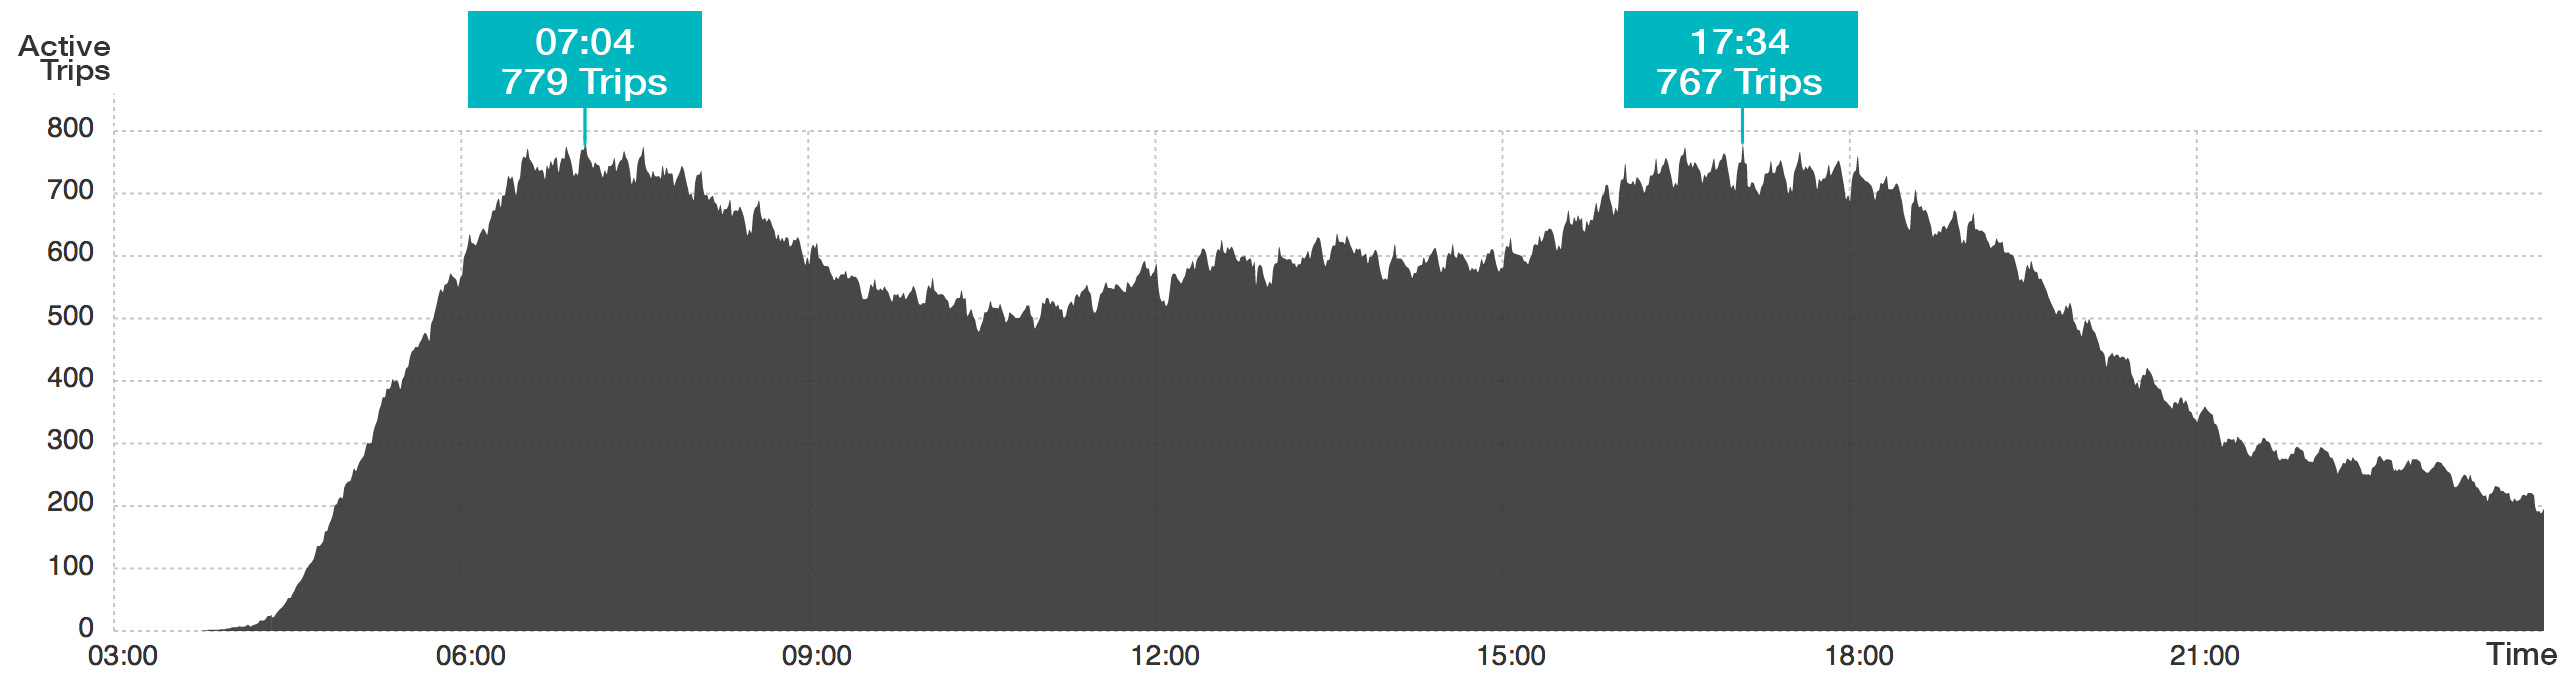
\includegraphics[width=\textwidth]{activeTrips.jpg}
      \caption{Anzahl an aktiven Trips zwischen 3.00 und 24.00 Uhr am 02.08.2017}
      \label{fig:activeTrips}
    \end{center}
  \end{figure}

  Anschließend flacht Mittags die Aktivität leicht ab, um dann zur Rush Hour am Abend wieder auf 767 gleichzeitig aktive Trips anzusteigen. Letztlich flacht die Anzahl immer weiter ab, um am nächsten Tag gegen 3 Uhr wieder anzusteigen und der Kreislauf beginnt von neuem. Insgesamt wurden an diesem Tag knapp 19650 Trips absolviert. Das Maximum betrug dabei $27 \frac{Trips}{Minute}$ wohingegen das Minimum bei $0 \frac{Trips}{Minute}$ lag. Im Schnitt starten 9 Vehicles pro Minute ihre Fahrt. Für eine interaktive Karte bedeutet dies, dass je nach Tag zwischen 0 und 1000 Trips aktiv sein können. Dies entspricht dann auch der Anzahl an Vehicle, die sich auf der Karte bewegen und animiert werden müssen. Sowohl durch die verschiedenen Frontend-Optimierungen aus Kapitel \ref{ssub:verbesserung_der_client_performance}, als auch durch die Anpassung von verschiedenen Bibliotheksfunktionen, konnte durchgängig ein Rendering mit 60 FPS im Frontend erreicht werden. Damit wurde dieses gesetzte Teilziel erreicht.\\

  Für die Ergebnisse der Evaluierung des Gesamtsystems wurden die Verarbeitungszeit des Servers, als auch die Antwortzeit der Datenbank in einem Zusammenhang betrachtet. Folgende Metriken lassen sich für dieses Gesamtsystem feststellen:

  \begin{longtable}{|>{\raggedright \arraybackslash}p{4.5cm}|>{\raggedright \arraybackslash}p{1.2cm}|>{\raggedright \arraybackslash}p{1.2cm}|>{\raggedright \arraybackslash}p{1.2cm}|>{\raggedright \arraybackslash}p{1.2cm}|>{\raggedright \arraybackslash}p{1.2cm}|>{\raggedright \arraybackslash}p{1.2cm}|}
  \caption{Backend Evaluation}\label{tbl:backend_evaluation}\\
    \hline
    Anz. Trips & 20 & 100 & 500 & 1000 & 5000 & 10000\\
    \hline
    Query Zeit (ms)        & 25 & 88 & 124 & 200 & 855 & 1631 \\
    Verarbeitungszeit (ms) & 2 & 27 & 40 & 142 & 226 & 435 \\
    Summe (ms)             & 27 & 115 & 164 & 342 & 1081 & 2066 \\
    \hline
  \end{longtable}

  In Tabelle \ref{tbl:backend_evaluation} sind die Datenwerte für verschiedene Abfragen aufgelistet. Die Werte ergeben sich aus dem Mittelwert der Laufzeit in 10 Durchläufen.\\

  Aus dieser Aussage plus den gemessenen Werten lässt sich folgende Schlussfolgerung ziehen: Bei einer Anzahl zwischen 20 und 100 Trips reagiert der Server innerhalb von 25 bis $120ms$. Da die meisten Trips in diese Spanne fallen, ist dieses Ergebnis am bedeutendsten. 

  Im Bereich von 100 bis 500 Trips ist eine Antwortzeit von 115 bis $164ms$ immer noch sehr gut. Diese Anzahl an Trips ist dann relevant, wenn die Applikation das erste Mal aufgerufen wird und die Karte noch leer ist. In diesem Fall kann es sein, dass der Server (je nach Datum und Uhrzeit) zwischen 200 - 500 Trips verarbeiten muss. Aber selbst Abfragen von bis zu 10.000 Trips, was ungefähr einer Zeitspanne von einem Tag gleich kommt, sind immer noch innerhalb von 2 Sekunden verarbeitet.\\

  Abschließend kann gesagt werden, dass in dieser Arbeit ein performantes Backendsystem für eine Web Applikation entwickelt worden ist, welches Serveranfragen effizient be- und verarbeiten kann.
  
% subsection ergebnisse (end)